\chapter{Perulangan (\textit{Looping})}

\section{Perulangan}
Perulangan dibutuhkan bilamana kita ingin mengeksekusi perintah yang sama berkali-kali dengan nilai yang berbeda maupun sama. Perulangan sering digunakan pada pemrosesan terhadap sekumpulan data, misalnya \textit{array}, \textit{list}, \textit{string} dan sebagainya.

\subsection{Struktur Perulangan}
Perulangan biasanya menggunakan pernyataan (\textit{for}) atau (\textit{while}). Pernyataan \textit{for} digunakan untuk mengiterasi sebuah \textit{array}, \textit{list} ataupun kumpulan variabel/objek lainnya sedangkan pernyataan \textit{while} digunakan untuk perulangan yang berdasarkan kondisi tertentu.

Struktur dari \textit{for} dalam pseudocode adalah sebagai berikut.
\begin{tabbing}
\textbf{for} $i=n$ \textbf{to} $m$~~~~~~~~~~~~~~~\=\#Mengisi variabel i, dan lakukan perulangan sebanyak (m-n-1)\\
~~~~~statements\\
\textbf{end for}
\end{tabbing}

\begin{contoh}
	\textbf{Penggunaan FOR}
	\begin{algorithm}
	\caption{PERULANGAN-FOR-CETAK-1-SAMPAI-5()}
		\begin{algorithmic}[1]
		\FOR{$i=1$ \TO $5$}
			\STATE print $i$
		\ENDFOR
		\STATE\COMMENT{Maka yang dicetak adalah 1 2 3 4 5}
		\STATE\COMMENT{Nilai $i$ terakhir yang tidak dicetak adalah 6}
		\end{algorithmic}
	\end{algorithm}
\end{contoh}

Dalam bahasa Python format \textit{for} adalah sebagai berikut.
\begin{tabbing}
\textbf{for} $i$ \textbf{in} $x$:~~~~~~~~~~~~~~~\=\#$x$ adalah \textit{kumpulan variabel}, iterasi dilakukan sebanyak panjang $x$\\
~~~~~statements\\
\end{tabbing}

Contoh penggunaan format Python untuk iterasi isi dari List bisa dilihat di Listing \ref{lst:iterasiArray}.
\begin{listprog}{iterasiList.py}
	\label{lst:iterasiArray}
	\begin{lstlisting}[language=Python]
		A = [4,1,3,5]
		for i in A:
			print i
		#Hasil print berupa 4 1 3 5
	\end{lstlisting}
\end{listprog}

Sedangkan untuk mencetak rangkaian bilangan misalnya dari 1 sampai 10 bisa menggunakan fungsi \textit{range}. Contohnya bisa dilihat di Listing \ref{lst:cetakBilangan}
\begin{listprog}{cetakBilangan.py}
	\label{lst:cetakBilangan}
	\begin{lstlisting}[language=Python]
		for i in range(1,11):
			print i
		#Hasil print berupa 1 2 3 4 5 6 7 8 9 10
	\end{lstlisting}
\end{listprog}

Untuk \textit{flowchart} \textit{for} bisa dilihat di Gambar \ref{fig:flowchartFor}.
\begin{figure}%
\centering
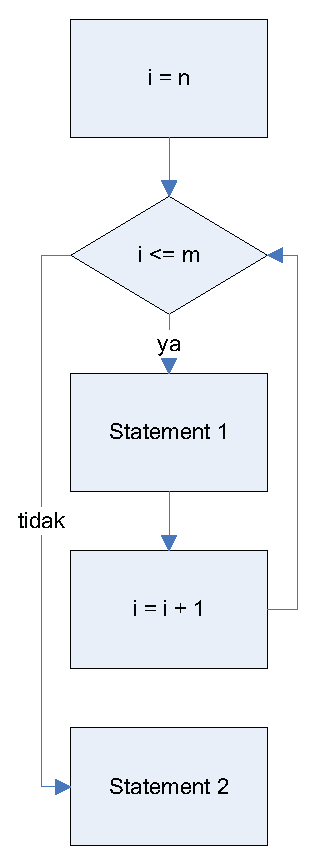
\includegraphics[scale=0.6]{fig/flowchart-FOR.eps}%
\caption{Flowchart For}%
\label{fig:flowchartFor}%
\end{figure}

\FloatBarrier
Untuk struktur \textit{while} bisa dilihat sebagai berikut.
\begin{tabbing}
\textbf{while} (Kondisi Logika)~~~~~~~~~~~~~~~\=\#Menjalankan perulangan selama kondisi benar\\
~~~~~statements\\
\textbf{end while}
\end{tabbing}

\FloatBarrier
\begin{contoh}
	\textbf{Penggunaan WHILE}
		\begin{algorithm}[H]
		\caption{PERULANGAN-WHILE-CETAK-1-SAMPAI-5()}
			\begin{algorithmic}[1]
			\STATE $i=1$
			\WHILE{$i<=5$}
				\STATE print $i$
				\STATE $i=i+1$
			\ENDWHILE
			\end{algorithmic}
		\end{algorithm}
\end{contoh}

Format bahasa Python untuk \textit{while} adalah sebagai berikut.

\begin{tabbing}
\textbf{while} (Kondisi Logika):~~~~~~~~~~~~~~~\=\#Menjalankan perulangan selama kondisi benar\\
~~~~~statements\\
\end{tabbing}

Contoh penggunaan \textit{while} dalam bahasa Python untuk mencetak menurun bilang 10 sampai 1 bisa dilihat di Listing \ref{lst:cetakBilanganTurun}.
\begin{listprog}{cetakBilanganTurun.py}
	\label{lst:cetakBilanganTurun}
	\begin{lstlisting}[language=Python]
		i = 10
		while(i>0):
			print i
			i = i - 1	\end
		#Hasil print berupa 10 9 8 7 6 5 4 3 2 1
	\end{lstlisting}
\end{listprog}


Untuk \textit{flowchart} \textit{while} bisa dilihat di Gambar \ref{fig:flowchartWhile}.
\begin{figure}%
\centering
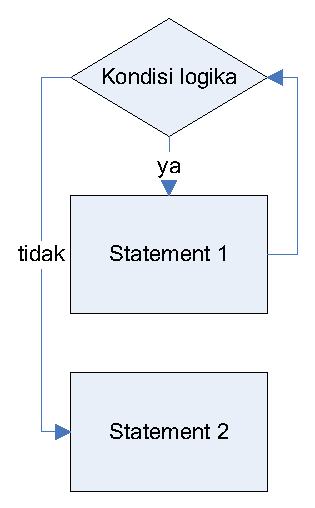
\includegraphics[scale=0.6]{fig/flowchart-WHILE.eps}%
\caption{Flowchart While}%
\label{fig:flowchartWhile}%
\end{figure}


\FloatBarrier
\subsection{Perulangan Bersarang}
Sebuah perulangan dapat memiliki perulangan di dalamnya dan perulangan yang di dalam tersebut juga dapat juga dapat memiliki perulangan lainnya di dalam. Perulangan yang di dalam tersebut tidaklah harus menggunakan pernyataan yang sama dengan perulangan induknya. Misalnya, boleh saja kita menggunakan pernyataan perulangan \textit{for} di dalam pernyataan perulangan \textit{while} dan juga sebaliknya. Algoritma berikut akan menunjukkan salah satu struktur perulangan bersarang.

\begin{tabbing}
\textbf{for} $i=n$ \textbf{to} $m$~~~~~~~~~~~~~~~\=\#Mengisi variabel i, dan lakukan perulangan sebanyak (m-n-1)\\
~~~~~\textbf{for} $j=n$ \textbf{to} $m$~~~~~~~~~~~~~~~\=\#Mengisi variabel j, dan lakukan perulangan sebanyak (m-n-1)\\
~~~~~statements\\
~~~~~\textbf{end for}\\
\textbf{end for}
\end{tabbing}

	
 
\section{Gabungan Percabangan dan Perulangan}
Dalam kondisi tertentu, suatu perulangan dapat memiliki percabangan di dalamnya. Biasanya percabangan di dalam perulangan digunakan untuk mengkhususkan perintah berbeda yang akan dikerjakan ketika variabel mencapai nilai tertentu. Pada perulangan yang memiliki percabangan di dalamnya, mungkin saja terdapat perintah :
\begin{enumerate}
	\item \textit{break}, yang akan menghentikan perulangan walaupun nilai varibelnya belum melampaui batas.
	\item \textit{continue}, yang akan melanjutkan perulangan ke tahapan perulangan berikutnya dan tidak akan menjalankan perintah di bawahnya.
\end{enumerate}
Dua contoh berikut akan menunjukkannya.

\begin{contoh}
	\textbf{Penggunaan BREAK}
	\begin{algorithm}
	\caption{PERULANGAN-CETAK-ANGKA-DENGAN-BREAK()}
		\begin{algorithmic}[1]
		\FOR{$i=1$ \TO $5$}
			\IF {$i == 4$}
				\STATE \textbf{break}
			\ENDIF
			\STATE print $i$
		\ENDFOR
		\STATE\COMMENT{Maka yang dicetak adalah 1 2 3.}
		\STATE\COMMENT{Pada saat $i$ mencapai nilai 4, perulangan langsung berhenti sebelum sempat mencetak.}
		\end{algorithmic}
	\end{algorithm}
\end{contoh}

\FloatBarrier
\begin{contoh}
	\textbf{Penggunaan CONTINUE}
	\begin{algorithm}
	\caption{PERULANGAN-CETAK-ANGKA-DENGAN-CONTINUE()}
		\begin{algorithmic}[1]
		\FOR{$i=1$ \TO $5$}
			\IF {$i == 4$}
				\STATE \textbf{continue}
			\ENDIF
			\STATE print $i$
		\ENDFOR
		\STATE\COMMENT{Maka yang dicetak adalah 1 2 3 5.}
		\STATE\COMMENT{Perulangan tetap akan dilanjutkan hingga i = 5, tanpa mencetak nilai 4.}
		\end{algorithmic}
	\end{algorithm}
\end{contoh}

\FloatBarrier
\begin{konsep}
\label{lat:pencetakanMatriks}
\textbf{Permasalahan pencetakan matriks}
Hasilkan sebuah algoritma dan \textit{flowchart} untuk mencetak matriks dengan ketentuan:
\begin{enumerate}
	\item Baris ganjil dari 1 sampai n
	\item Baris genap dari n turun sampai 1
\end{enumerate}
\textbf{Masukan}\\
Sebuah bilangan bulat $n$.\\ 
\textbf{Keluaran}\\
Keluarannya berupa matriks $n$x$n$ dengan baris ganjil merupakan rangkaian angka menaik dari 1 sampai n dan baris genap merupakan rangkaian angka menurun dari n sampai 1.\\
\begin{center}
\textbf{Test Case 1}\\
\end{center}
\textbf{Masukan}\\
5\\
\textbf{Keluaran}\\
1 2 3 4 5 \\
5 4 3 2 1 \\
1 2 3 4 5 \\
5 4 3 2 1 \\
1 2 3 4 5 \\
\begin{center}
\textbf{Test Case 2}\\
\end{center}
\textbf{Masukan}\\
3\\
\textbf{Keluaran}\\
1 2 3 \\
3 2 1 \\
1 2 3 \\
\end{konsep}

\begin{pemrograman}
Buatkan program python dari Latihan \ref{lat:pencetakanMatriks}.
\end{pemrograman}

\begin{konsep}
\label{lat:pencetakanBintang}
\textbf{Permasalahan pencetakkan bintang dari NIM}\\
Hasilkan algoritma dan \textit{flowchart} untuk mencetak bintang dan angka berikut dengan menggunakan NIM sebagai dasarnya.\\
\textbf{Masukan}\\
Sebuah \textit{String} 9 karakter dimana merupakan NIM dari mahasiswa STMIK Mikroskil.\\
\textbf{Keluaran}\\
9 baris dimana di baris i terdapat karakter i, satu spasi dan diikuti bintang sejumlah karakter i tersebut.\\
\begin{center}
\textbf{Test Case 1}\\
\end{center}
\textbf{Masukan}\\
121114567\\
\textbf{Keluaran}\\
1 * \\
2 ** \\
1 * \\
1 * \\
1 * \\
0 \\
5 ***** \\
6 ****** \\
7 ******* \\
\begin{center}
\textbf{Test Case 2}\\
\end{center}
\textbf{Masukan}\\
031110023\\
\textbf{Keluaran}\\
0  \\
3 *** \\
1 * \\
1 * \\
1 * \\
0 \\
0 \\
2 ** \\
3 *** \\
\end{konsep}

\begin{pemrograman}
Buatkan program python dari Latihan \ref{lat:pencetakanBintang}.
\end{pemrograman}